The analysis strategy follows the same steps described in Section 3. Due to the lower statistics available, due to the centrality slicing, the transverse momentum ranges of associated tracks are reduced to the following three: $\pt^{\rm assoc}>0.3$ $\gev/c$, $0.3<\pt^{\rm assoc}<1$ $\gev/c$, $\pt^{\rm assoc}>0.3$ $\gev/c$. No variations are instead done for the four D-meson $\pt$ ranges: $3<\pt^{\rm trig}<5$ $\gev/c$, $5<\pt^{\rm trig}<8$ $\gev/c$, $8<\pt^{\rm trig}<16$ $\gev/c$, $16<\pt^{\rm trig}<24$ $\gev/c$ (the last bin already suffers by statistics issues).

\subsubsection{Dataset and event selection}
The data samples and Monte Carlo productions exploited for the analysis are the same as those for the cent-integrated studies, i.e. LHC16q$+$LHC16t (FAST and CENT$\_$wo$\_$SDD samples, granting a better uniformity along $\varphi$ and $\eta$) for data and LHC17d2a$\_$fast$\_$new (HF enriched) and LHC17f2b$\_$cent$\_$woSDD,$\_$fast (minimum-bias) for Monte Carlo.
The list of runs studied in the analysis is also the same as that showed in Table 1.
In addition to the previous event selection, described in Section 2, there is an additional requirements for the centrality slicing: the ZNA estimator is employed to slice the data sample in three complementary centrality classes (0-20\%, 20-60\%, 60-100\%). The chosen slicing grants substantial differences, in terms of average centrality, between the first and the third class, and also allows to fairly equalize the number of D-mesons in each class (since the second and third classes are wider, but also have a lower N$_{coll}$ value w.r.t. the first).

The number of analyzed events for the three is approximately:
\begin{itemize}
  \item 123M for 0-20\% centrality
  \item 247M for 20-60\% centrality
  \item 246M for 60-100\% centrality
\end{itemize}

The possibility of using the V0A estimator was also studied - and fully-corrected results for V0A estimator are also available - but the final choice of the centrality estimator fell on the ZNA. Indeed, this estimator is more directly related to the collision geometry than the V0A, which is instead more pointed toward a tagging of the event multiplicity.

\subsubsection{Mass plots and D-meson selection}
The topological selection is largely based on the cut values used for the cent-integrated analysis.
For the $\Dzero$, a specific cut optimization in each centrality class was performed, but tightening/loosening the cut values and checking the performance in terms of statistical uncertainties on the background-subtracted azimuthal correlation distributions.
Some small gain (about 5\% to 10\% depending on the kinematic range) were obtained by:
\begin{itemize}
  \item tightening the cosine of pointing angle for the 0-20\% centrality
  \item slightly loosening the the cosine of pointing angle and slightly tightening the normalized $L_{xy}$  for 20-60\% centrality
  \item loosening the cosine of pointing angle for the 60-100\% centrality
\end{itemize}
A similar optimization was also tried for the $\Dplus$ and $\Dstar$ mesons, but no gains were obtained, hence the cent-integrated selection was applied.

\textit{\textbf{SHOW THE MASS PLOTS FOR THE THREE D-MESONS (A SELECTION!)}}

As from the standard procedure (described in details in Section 3), bidimensional ($\Delta\eta$,$\Delta\varphi$) correlation distributions are built for D-meson candidates found in the signal region and in the sidebands, and the sidebands correlations, after a proper normalization, are subtracted from the signal region correlations to remove the contribution from the correlations from D-meson combinatorial background under the peak. The definition of the signal region and sideband does not change with respect to the centrality-integrated analysis.

\subsubsection{Event mixing}
The correction for limited acceptance of the detector, and its local inefficiencies, follows exactly the same procedure enonuced in subsection 3.3.1.
The only small difference deals with the definition of the multiplicity ranges of the 9 mixed events pools. Since the three centrality classes contain event with different SPD tracklet multiplicity distributions, a modification of these ranges was required to balance the number of events entering in each mixed event pool, as follows:
\begin{itemize}
  \item {0,55,80,500} for 0-20\% centrality
  \item {0,35,55,500} for 20-60\% centrality
  \item {0,20,30,500} for 60-100\% centrality
\end{itemize}

\subsubsection{Tracking and trigger efficiency}

{\bf (i) Tracking efficiency}

The associated track efficiency is based on an online weighting of the D-meson and associated track correlation pairs, by means of a three-dimensional efficiency map, as described in details in subsection 3.3.2 (i).
The same efficiency.
This choice was based on the fact that no variations on the associated track cuts was performed between the two analyses, so the efficiency is not varied, and that there is a negligible dependence of the tracking efficiency on the event centrality/multiplicity.
The latter assumption was checked by evaluating tracking efficiency maps for each centrality slice, i.e. running the tracking efficiency task on a sample of Monte Carlo reproducing the same event multiplicity distributions (in terms of SPD tracklets) observed on data for each slice.

The event weights applied to the Monte Carlo events to mimick each centrality slice (as well as those to reproduce the same multiplicity also for the centrality-integrated sample) are shown in Fig. \ref{fig:Weights}. They are presented for both ZNA and V0A estimator. As it is evident, the V0A tends to favour more high-multiplicity events for the 0-20\% centrality class, and low-multiplicity events for the 60-100\%; the ZNA estimator instead equalizes more the event multiplicity distribution in the three centrality slices.

\begin{figure}
\centering
{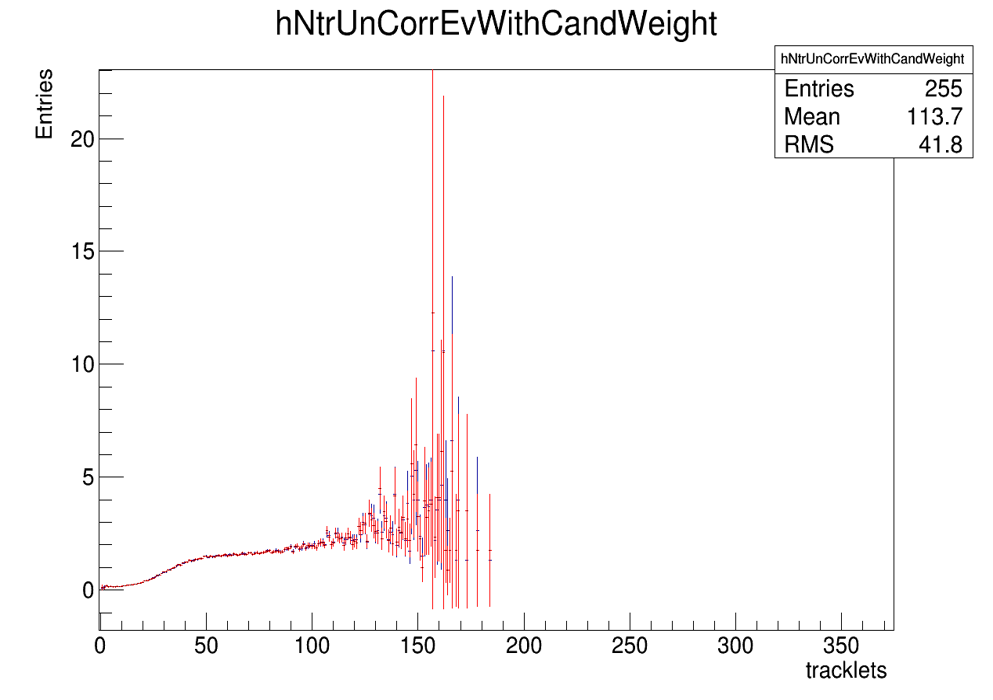
\includegraphics[width=0.4\linewidth]{figuresVsCent/Global/Weight0100.png}}
{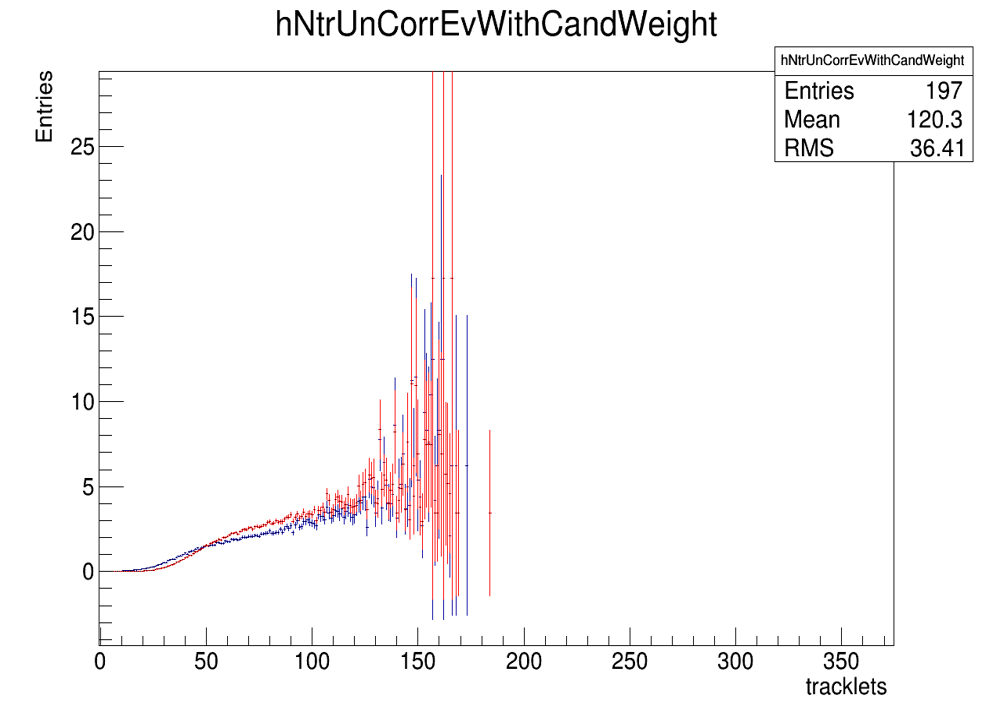
\includegraphics[width=0.4\linewidth]{figuresVsCent/Global/Weight020.png}} \\
{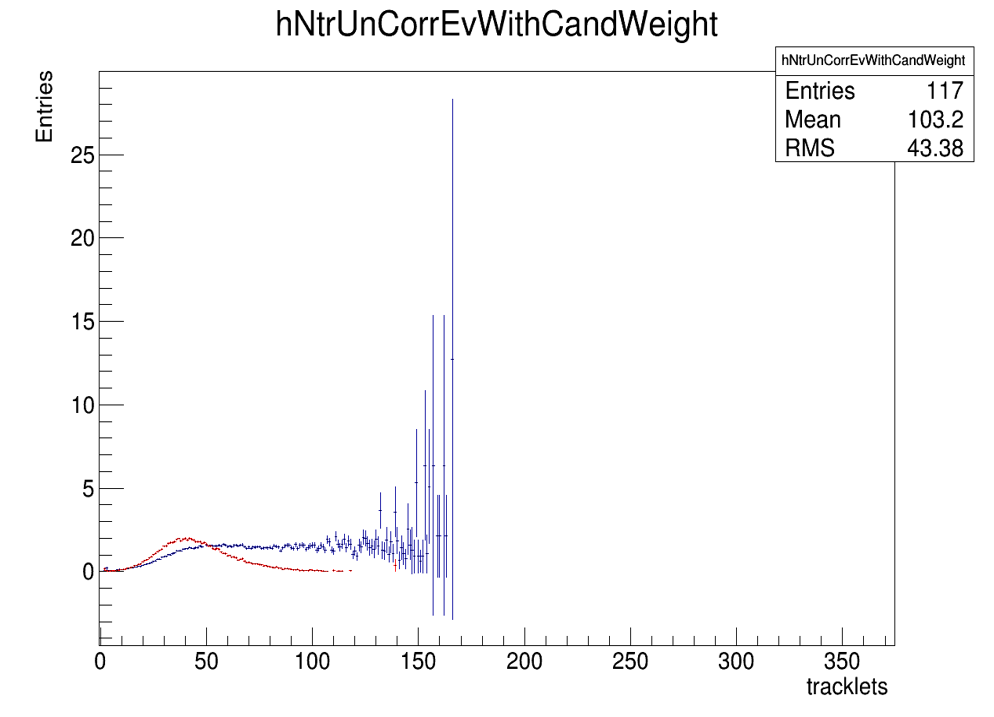
\includegraphics[width=0.4\linewidth]{figuresVsCent/Global/Weight2060.png}}
{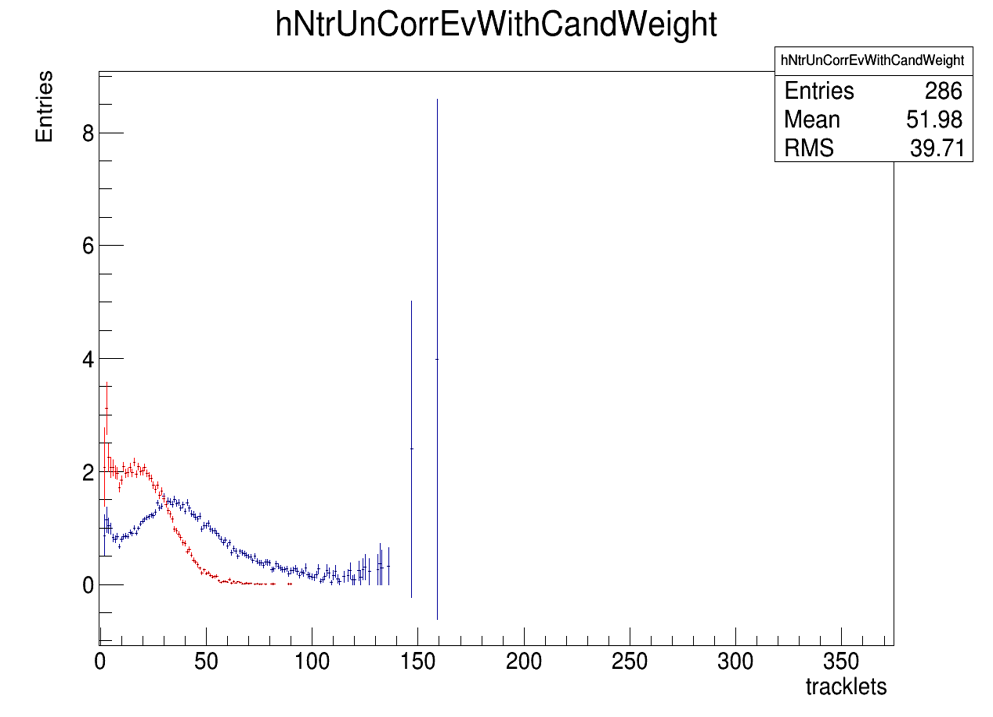
\includegraphics[width=0.4\linewidth]{figuresVsCent/Global/Weight60100.png}}
 \caption{Event weights applied to Monte Carlo sample, to mimic the multiplicity distribution for centralities: 0-100\% (cent-integrated), 0-20\%, 20-60\%, 60-100\%. Blue points are for ZNA, red points for V0A estimator.}
\label{fig:Weights}
\end{figure}

After comparing the tracking efficiency maps evaluated applying the event weights on the monte Carlo events, with those obtained running on the unweighted Monte Carlo sample, differences of the order of few per mille were found, confirming the possibility of using the same tracking efficiency map for the various centrality slices.
As an example, the ratio of $\pt$-projection of the tracking efficiency maps when 0-20\% weights are applied and where no weights are applied on the events is shown in Fig. \ref{fig:TrackEFfWeights}, and it results to be fully compatible with 1.

\begin{figure}
\centering
{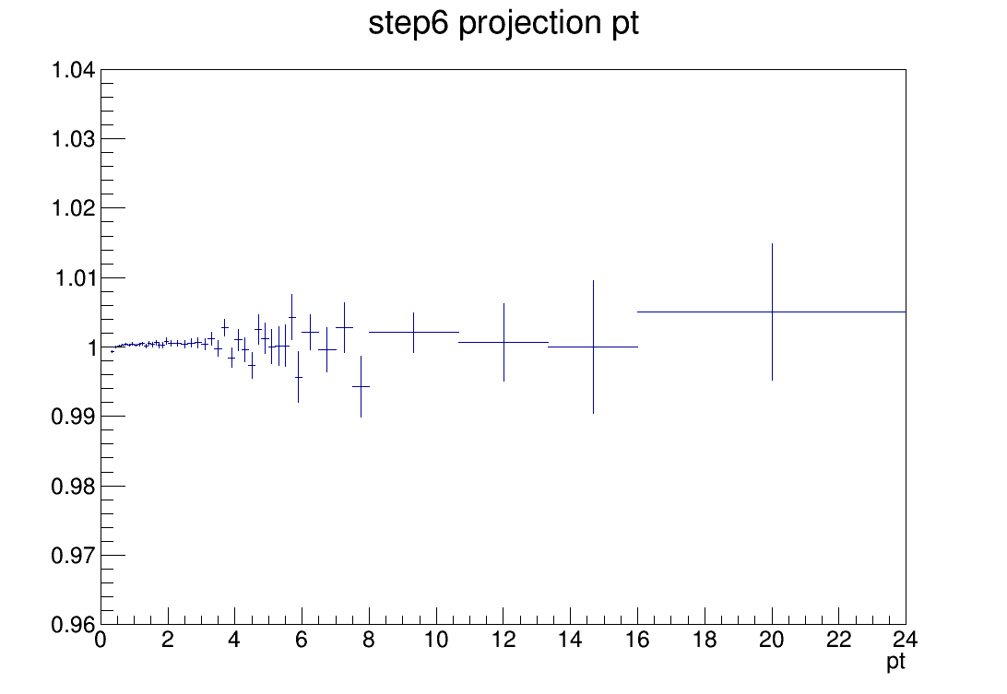
\includegraphics[width=0.7\linewidth]{figuresVsCent/Global/CrossCheck_TrackEffWeight.png}}
 \caption{Ratio of 1D track efficiency map vs $\pt$ with and without event weights (excample for 0-20\%) applied on the Monte Carlo sample.}
\label{fig:TrackEFfWeights}
\end{figure}

{\bf (ii) Trigger efficiency}

Differently from the track efficiency, the D-meson reconstruction and selection efficiency can have a dependence on the event multiplicity that has to be taken into account. This mainly depends on the lower efficiency on the reconstruction of the primary vertex (included in the overall D-meson reconstruction efficiency) for very low multiplicity events. Indeed, as it can be seen in Fig. {\bf REF}, the efficiency is rather flat above 20-30 tracklets, and starts to drop below that SPD tracklet multiplicity.

\textit{\textbf{INSERT THE PLOT OF 1D EFFICIENCY VS MULTIPLICITY! I THINK DPLUS OR DSTAR HAVE ONE.}}

To consider this dependence, separate trigger efficiency maps were built for each centrality slice, by running the trigger efficiency task on the reweighted Monte Carlo enriched sample (using the same event weights described above).
In Fig. {\bf REF} the trigger efficiency maps, and their projection onto the $\pt$ axis, are shown for the three D mesons in each centrality class considered.

\textit{\textbf{SHOW THE TRIGGER EFF MAPS (2D and possibly 1D, ONLY FOR CHARM ORIGIN!) FOR THE 3 MESONS AND FOR THE 3 CENTRALITIES!}}

Then, the trigger efficiency correction follows the same procedure, based on an online-weighting of the correlation pairs, described in subsection 3.3.2 (ii).

\subsubsection{Correction for bias on B to D decay topologies}
As described in detail in subsection 3.3.3, performing a Monte Carlo closure test allows to spot a bias on the correlation distributions, due to the presence of structures in the near-side region for B$\rightarrow$D-h correlations, induced by the topological selection on the D.
After the projection of the correlation distributions on $\Delta\varphi$, a correction has thus to be applied on the azimuthal correlation distributions. The procedure for the evaluation of the correction to apply on data is repeated for each centrality class.
The outcome of the MC closure test, i.e. the Reco/Kine ratios, is shown for each centrality class in Fig. {\bf REF} (using the $\Dzero$ meson as trigger).

\textit{\textbf{SHOW THE MC CLOSURE TEST FOR THE 3 CENTRALITIES!}}

As (slightly) visible from the plots, the B$\rightarrow$D structures are larger in 0-20\% rather than in 60-100\% if only the associated tracks coming from beauty are considered (light-green point). Anyway, the situation is reversed when considering all the associated tracks, i.e. also the uncorrelated pairs (dark-green points) - which is the case to be considered to evaluate the correction. This is understandable, due to the lower presence of uncorrelated pairs in 60-100\%, which enhances the peak/baseline ratio w.r.t. 0-20\%. This also reflects in a (slightly) larger correction for 60-100\% centrality class rather than for 20-60\% and 0-20\%.
Anyway, the overall correction applied on data (following Equation 3) is always lower than 3\%, even for the worst case, being the lowest D-meson $\pt$ bin ($3 < \pt < 5$ GeV/$c$) and the highest associated track $\pt$ bin ($\pt > 1$ GeV/$c$).
Furthermore, the difference of the correction values among the different centrality classes is never larger than 1.5\%.

\subsubsection{Secondary track contamination}
The strategy for the the purity correction and the Monte Carlo study for its quantitative evaluation are similar to that described in subsection 3.3.4.
A major improvement was introduced for the centrality-dependent analysis: the correction for removing the secondary tracks passing the associated track selection is not anymore performed as a global scale factor of the correlation distributions (i.e. flat in $\Delta\varphi$), but is now performed differentially along the azimuthal axis (i.e. applied bin-per-bin on the azimuthal correlation distributions).
This choice was done because, from the Monte Carlo analysis, the contamination of secondary particles in the selected track sample (or, in a complementary view, the purity) is not completely flat in $\Delta\varphi$, but shows some structures, in particular in the near-side region. Some examples are shown in Fig. \ref{fig:Purity} (blue histogram), where the fraction of primary track vs $\Delta\varphi$ is shown for exemplary kinematic regions.

\begin{figure}
\centering
{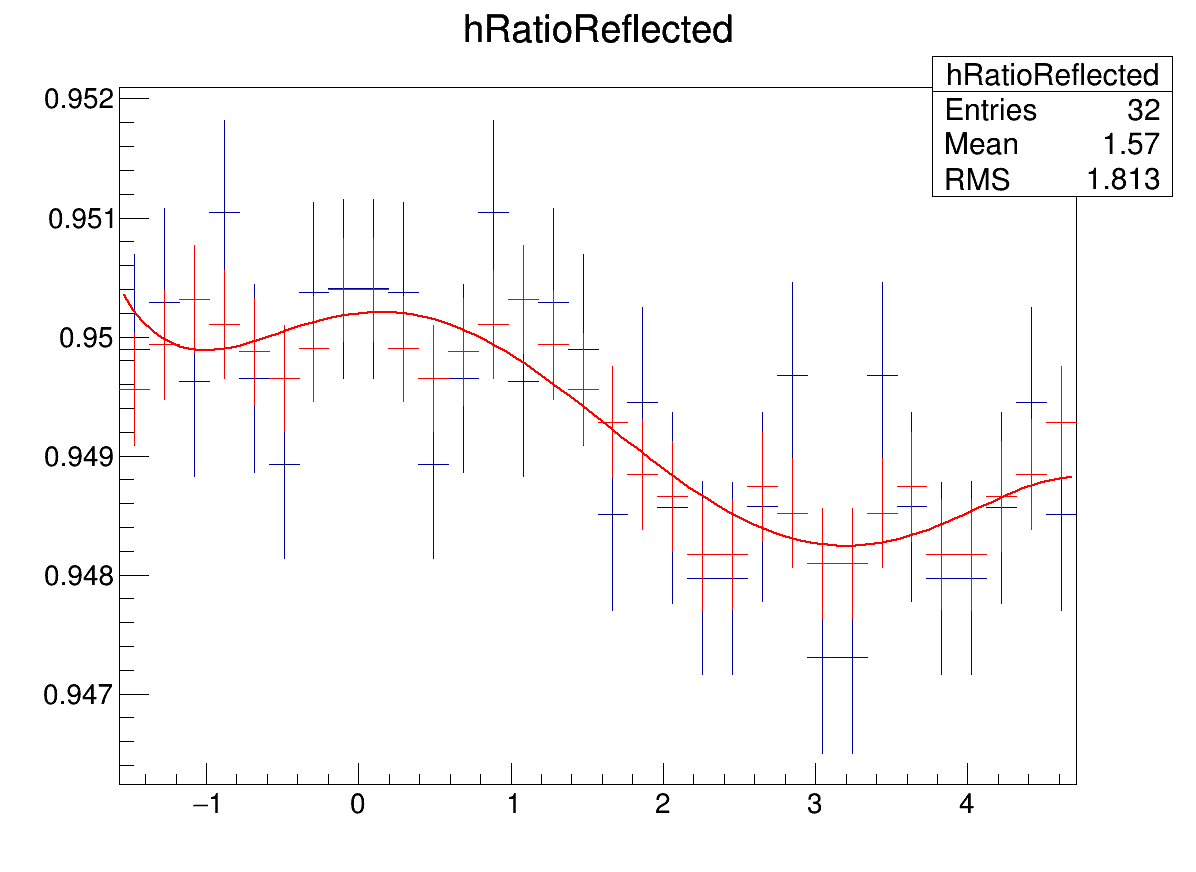
\includegraphics[width=0.4\linewidth]{figuresVsCent/Global/Purity/DeltaPhi_3to5_03to1_RatioPrimOverAll.png}}
{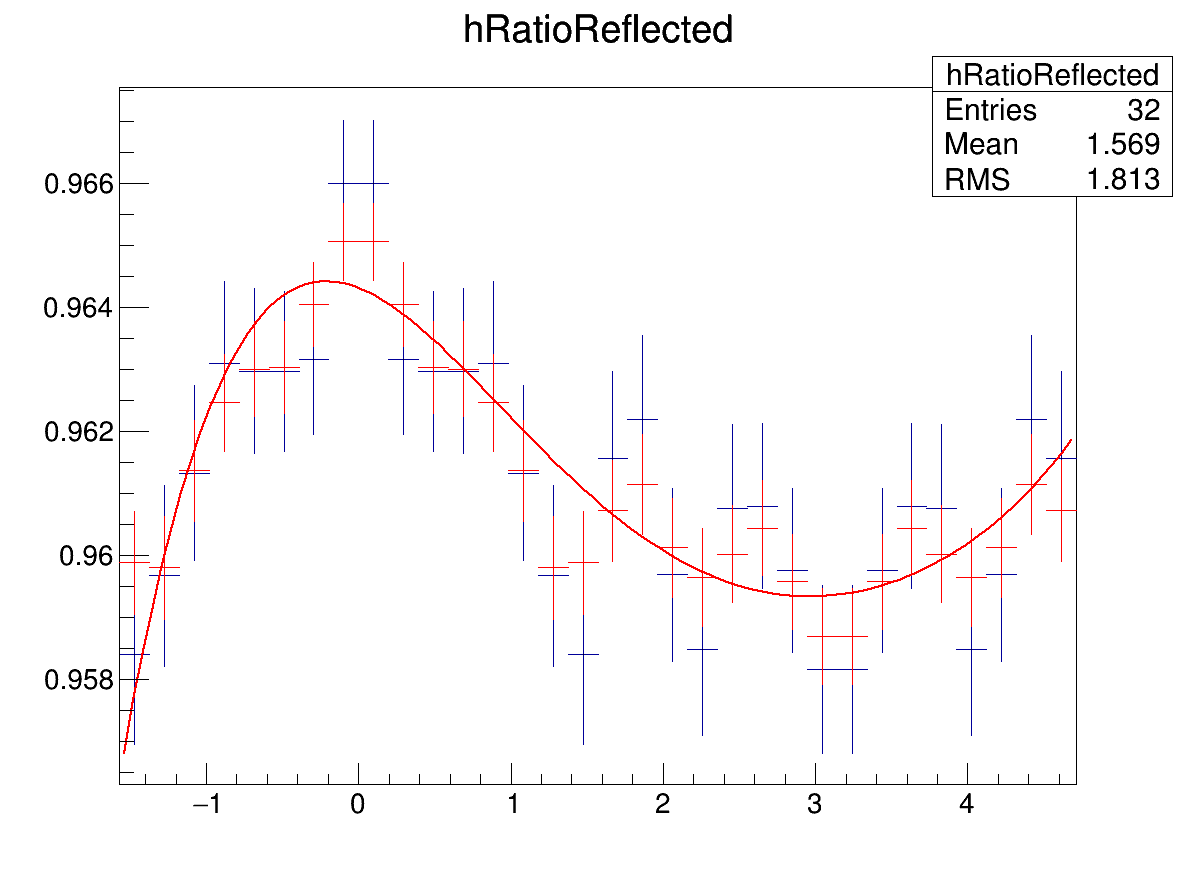
\includegraphics[width=0.4\linewidth]{figuresVsCent/Global/Purity/DeltaPhi_3to5_1to99_RatioPrimOverAll.png}} \\
{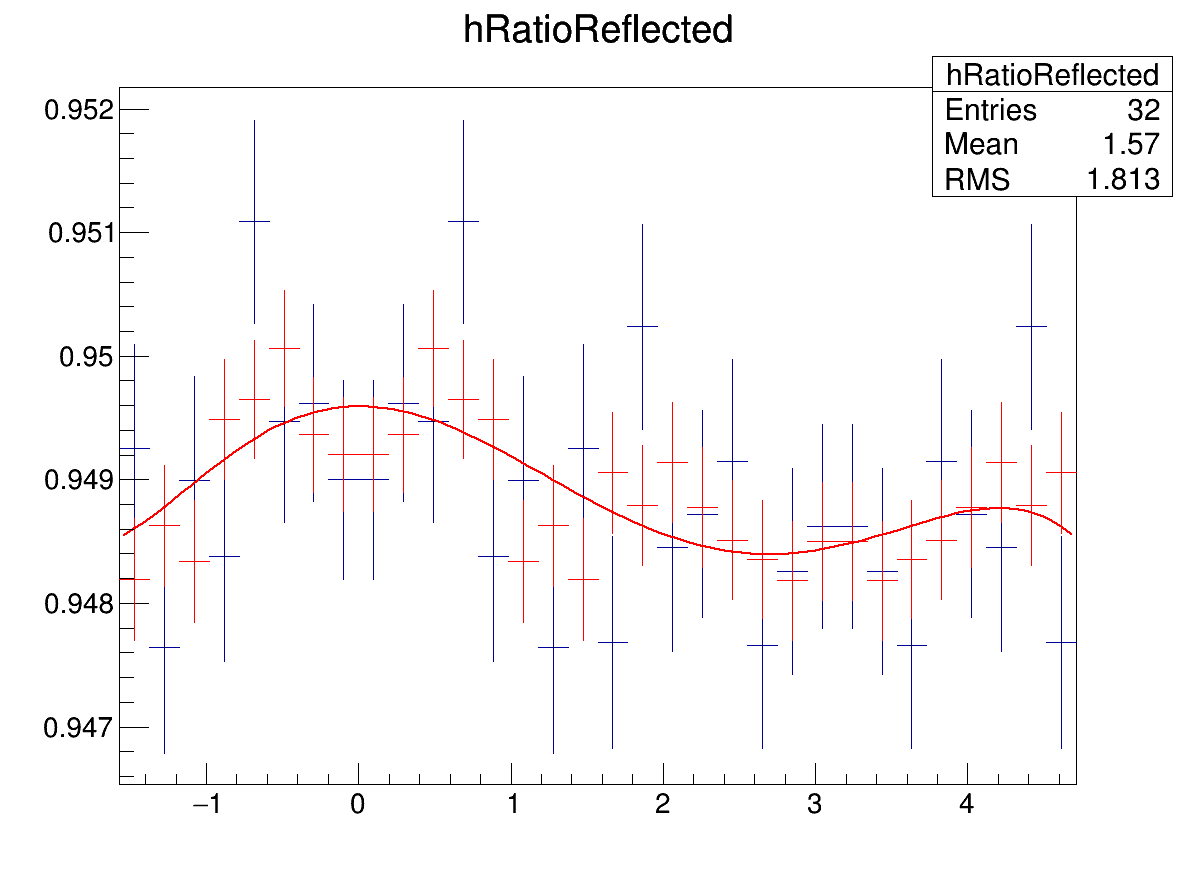
\includegraphics[width=0.4\linewidth]{figuresVsCent/Global/Purity/DeltaPhi_5to8_03to1_RatioPrimOverAll.png}}
{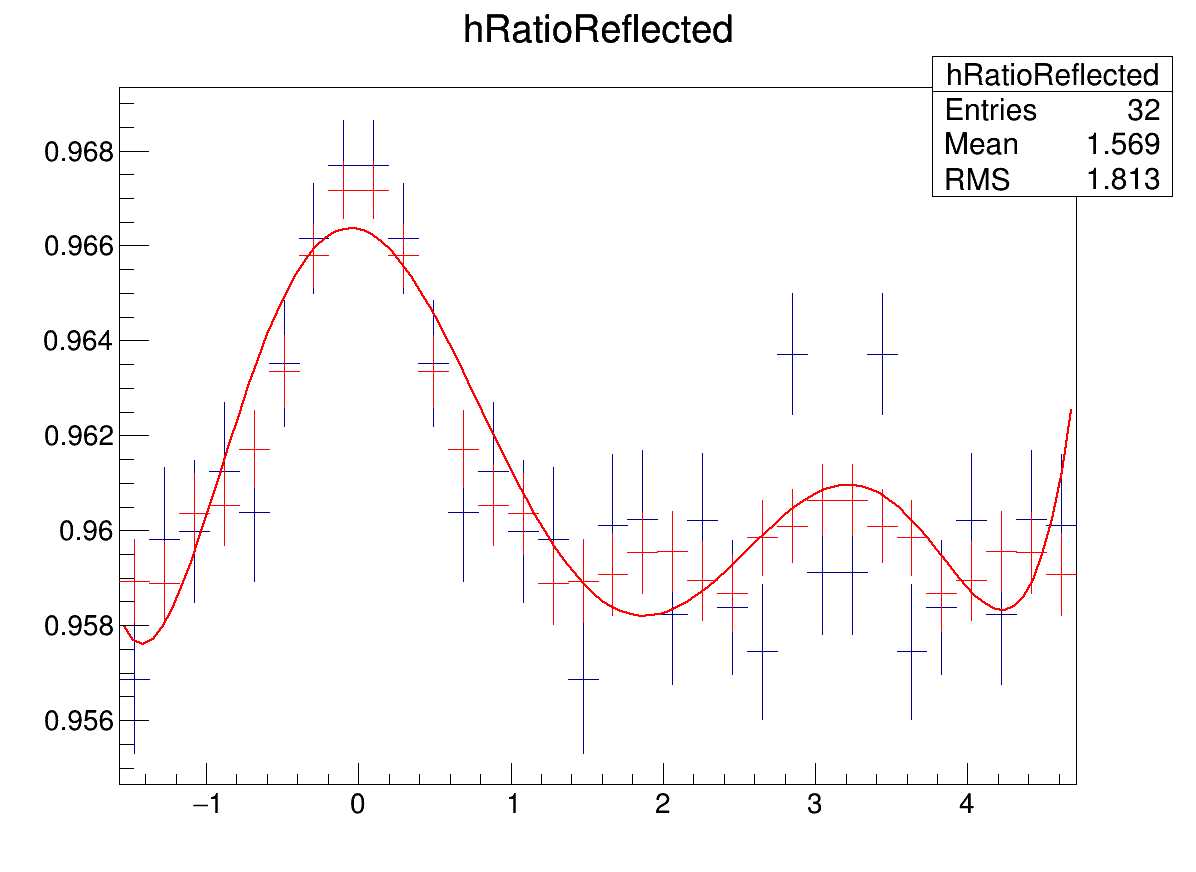
\includegraphics[width=0.4\linewidth]{figuresVsCent/Global/Purity/DeltaPhi_5to8_1to99_RatioPrimOverAll.png}} \\
{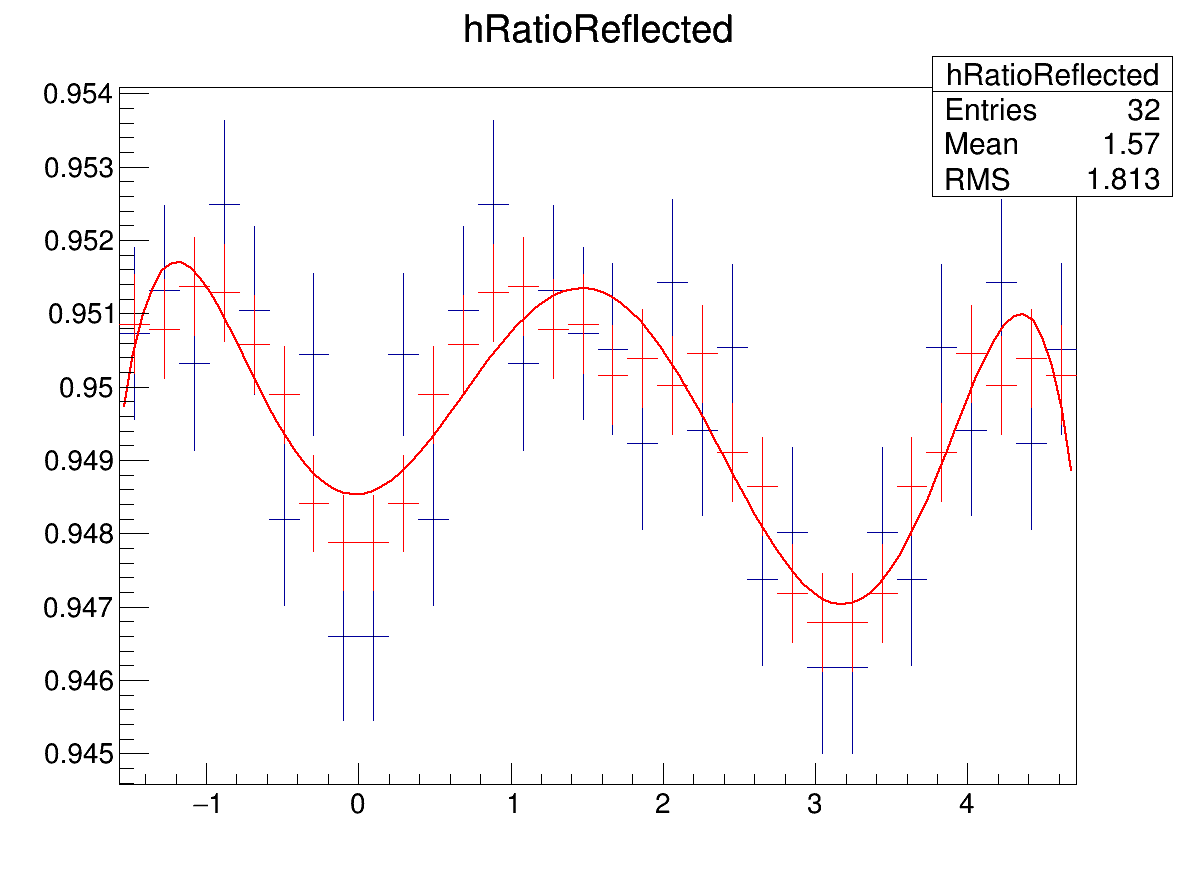
\includegraphics[width=0.4\linewidth]{figuresVsCent/Global/Purity/DeltaPhi_8to16_03to1_RatioPrimOverAll.png}}
{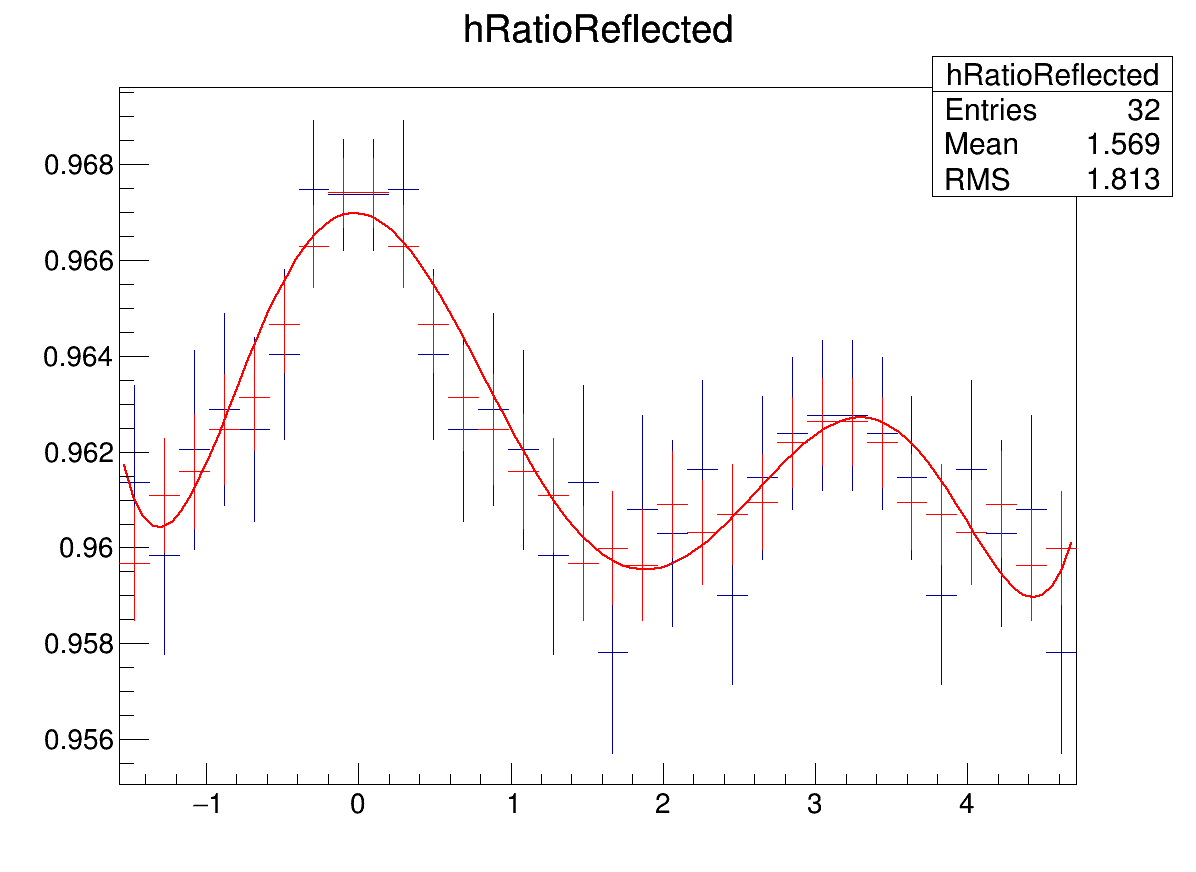
\includegraphics[width=0.4\linewidth]{figuresVsCent/Global/Purity/DeltaPhi_8to16_1to99_RatioPrimOverAll.png}}
 \caption{Fraction of primary track in the reconstructed associated track sample (blue histogram). The polynomial fit function (red curve) and the 3-point moving average (red histogram) are also superimposed. The $\pt$(D) ranges are 3-5, 5-8, 8-16 GeV/$c$, respectively for each row, and $0.3 < \pt$(assoc)$ < 1$, $\pt$(assoc) $> 1$ GeV/$c$ inside each row. }
\label{fig:Purity}
\end{figure}

Though these structures are small (about 1\%), they could be amplified after the subtraction of the baseline, when going to the yield evaluation. For this reason, the $\Delta\varphi$-differential correction was chosen implemented.
In particular, three approaches were tried, by multiplying the data correlation distribution by:
\begin{itemize}
  \item the MC primary/inclusive histogram (blue histogram in Fig. \ref{fig:Purity})
  \item a polynomial fit applied to the MC primary/inclusive histogram (red curve in Fig. \ref{fig:Purity})
  \item a moving average, considering 3 points, of the MC primary/inclusive histogram (blue histogram in Fig. \ref{fig:Purity})
\end{itemize}
Each approach has pros and cons, since directly using the primary/inclusive histogram gives a correction strongly dependent on the statistical fluctuations, while using the fit or the moving average smoothen the fluctuation, but also the structures with a physical origin.
For this reason, a comparison of the outcome of the correction after applying either of the approaches (and the old 'flat' correction approach) was performed.
The results of the check is shown in Fig. \ref{fig:PurityAppr}, for $3<\pt^{\rm trig}<5$ $\gev/c$ (situation is identical in the other D-meson $\pt$ ranges). The difference of the new approaches w.r.t. the flat one is around 1\% at maximum (under the near-side, for $\pt$(assoc) $> 1$ GeV/$c$, while the outcome of the correction is completely equivalent when using either of the new approaches.

\begin{figure}
\centering
{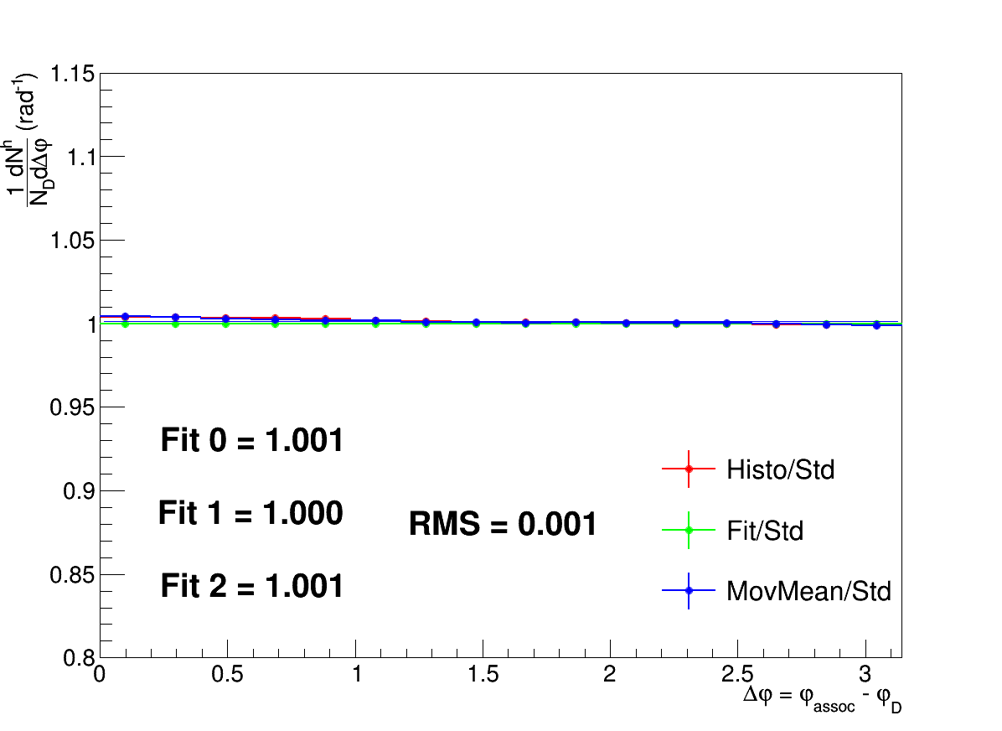
\includegraphics[width=0.45\linewidth]{figuresVsCent/Global/Purity/PurityCheck1.png}}
{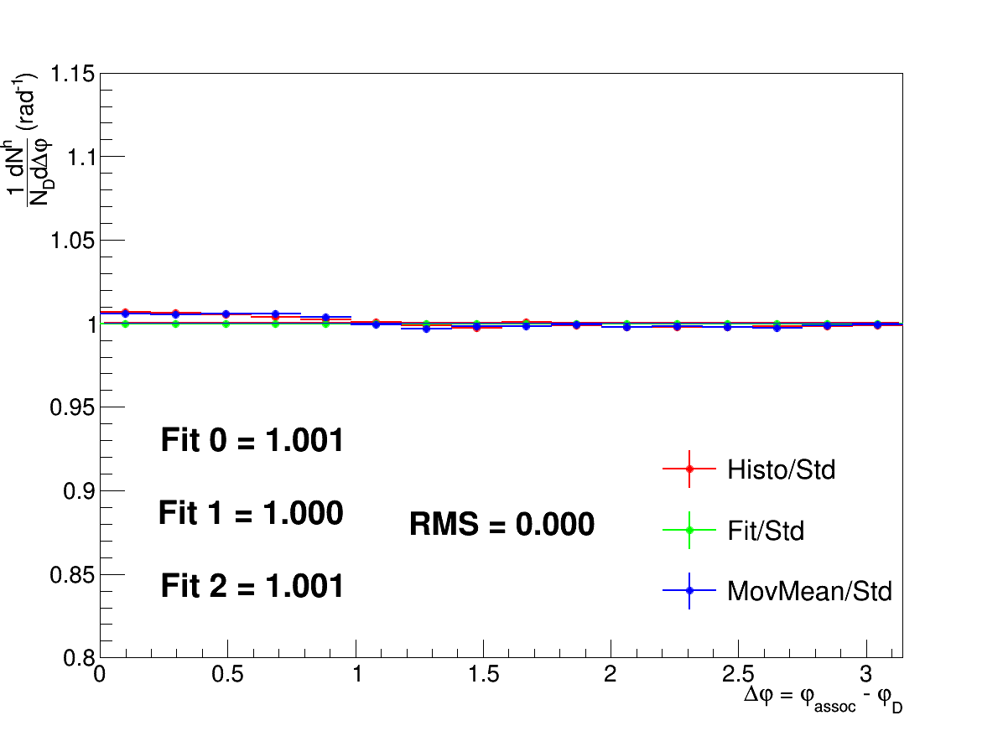
\includegraphics[width=0.45\linewidth]{figuresVsCent/Global/Purity/PurityCheck2.png}} \\
{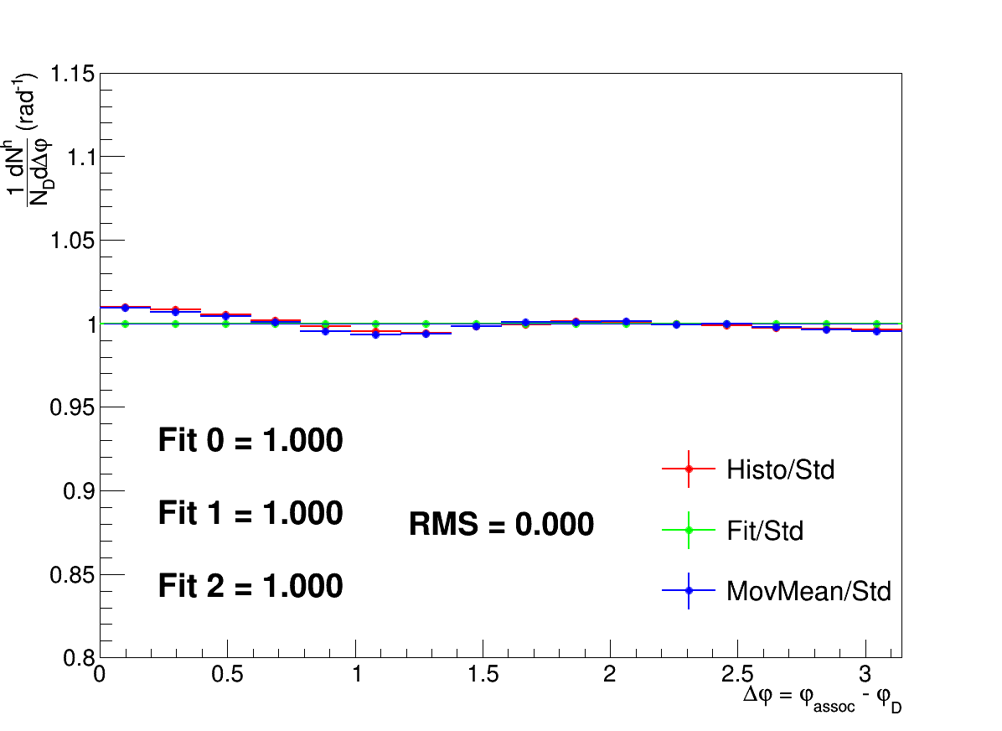
\includegraphics[width=0.45\linewidth]{figuresVsCent/Global/Purity/PurityCheck3.png}}
 \caption{Ratio of correlation distribution after purity correction with $\Delta\varphi$ differential correction over those with flat purity correction, for the three associated $\pt$ ranges in $\pt$(D) 3-5 GeV/$c$.}
\label{fig:PurityAppr}
\end{figure}

The correction was independently evaluated on each centrality class (by applying the event weights to the Monte Carlo).
No significant deviations of the purity were found among the different centralities.
As an example, Fig. {\bf REF} shows the average purity contribution (linear fit over the distributions of slide), for the various kinematic regions, for each centrality class. The same conclusion holds also for the differential correction, effectively applied on data.

\textit{\textbf{SHOW THE (FLAT) PURITIES FOR THE 3 CENTRALITIES!}}

\subsubsection{Feed-down correction}
The technique for performing the feed-down correction is based on the subtraction of templates of correlation distributions of feed-down D- and charged particle correlations obtained from Monte Carlo simulations - after their rescaling by means of the fraction of prompt D meson in the reconstructed D-meson sample, f$\_{\rm prompt}$.
The procedure fully coincides to that used for the cent-integrated analysis, described in details in subsection 3.3.5.
The only modification consists in a possible dependence of the feed-down correction on the centrality of the event, for the following reasons:
\begin{itemize}
  \item Variation of D-meson efficiency vs centrality, due to the lower primary vertex reconstruction efficiency at low multiplicity and, for $\Dzero$, to centrality-dependent topological cut values. This, in turn, impacts on f$\_{\rm prompt}$ because of its dependence on the D-meson efficiency.
  \item Possible variation of $R_{\rm pPb}$(B)/$R_{\rm pPb}$(D), on which f$\_{\rm prompt}$ depends, on the centrality of the event.
  \item Dependence of the B$\rightarrow$D-hadron correlation peaks on the event centrality. This would require modifying the MC templates for B$\rightarrow$D-hadron correlations used for each centrality class. This effect was neglected, since no evidences exist, at the moment, on a possible modification of the heavy-flavour quark fragmentation versus the event multiplicity.
\end{itemize}
To consider the above effects, an independent evaluation of f$_{\rm prompt}$ was performed in each centrality class, using the specific trigger efficiency maps and possible ranges of $R_{\rm pPb}$(B)/$R_{\rm pPb}$(D) (entering in the f$\_{\rm prompt}$ uncertainty), from 0.9-1.1 in 60-100\% to 0.9-1.3 in 0-20\%.
The resulting f$\_{\rm prompt}$ values are shown, for the three D mesons, in Fig. {\bf REF}.

\textit{\textbf{SHOW THE FPROMPT FOR THE 3 CENTRALITIES!}} 